%---------DO NOT EDIT THIS INDENTED SECTION
	% Preamble
	\documentclass[11pt,reqno,oneside,a4paper]{article}
	\usepackage[a4paper,includeheadfoot,left=35mm,right=35mm,top=00mm,bottom=30mm,headheight=40mm]{geometry} %sets up the margins
	\usepackage{graphicx}
	\graphicspath{{./images/}}
	\setlength{\parindent}{0pt}
	%%%%%%%%%%%%%%%%%%%%%%%%%%%%%%%%%%%%%%%%%%%%%%%%%%%%%%%%%%%%%%%%%%%%%%%%%%%%%%%%
%
% This file contains some standard modifications to basic LaTeX2e and
% the article documentclass. DO NOT EDIT THIS FILE, but do look through
% and make use of the shorthands defined herein.
%
%%%%%%%%%%%%%%%%%%%%%%%%%%%%%%%%%%%%%%%%%%%%%%%%%%%%%%%%%%%%%%%%%%%%%%%%%%%%%%%%

% Standard packages
\usepackage{amssymb,amsmath,amsthm}
\usepackage{xcolor,graphicx}
\usepackage{verbatim}
\usepackage{hyperref}
% Layout of headers & footers
\usepackage{titling}
\usepackage{fancyhdr}
\pagestyle{fancy} \lhead{{\theauthor}} \chead{} \rhead{} \lfoot{} \cfoot{\thepage} \rfoot{}

% Hyphenation
\hyphenation{non-zero}

% Instructor's email address
\newcommand{\InstEmail}{fspagnuolo@yale-nus.edu.sg}

%% Mathmode shortcuts
% Number sets
\newcommand{\NN}{\mathbb N}              % The set of naturals
\newcommand{\NNzero}{\NN^0}              % The set of naturals including zero
\newcommand{\NNone}{\NN}                 % The set of naturals excluding zero
\newcommand{\ZZ}{\mathbb Z}              % The set of integers
\newcommand{\QQ}{\mathbb Q}              % The set of rationals
\newcommand{\RR}{\mathbb R}              % The set of reals
\newcommand{\CC}{\mathbb C}              % The set of complex numbers
\newcommand{\KK}{\mathbb K}              % An arbitrary field
% Modern typesetting for the real and imaginary parts of a complex number
\renewcommand{\Re}{\operatorname*{Re}} \renewcommand{\Im}{\operatorname*{Im}}
% Upright d for derivatives
\newcommand{\D}{\ensuremath{\,\mathrm{d}}}
% Make epsilons look more different from the element symbol
\renewcommand{\epsilon}{\varepsilon}
% Always use slanted forms of \leq, \geq
\renewcommand{\geq}{\geqslant}
\renewcommand{\leq}{\leqslant}
% Shorthand for some relations
\newcommand{\po}{\preceq}
\newcommand{\rel}{{\mathcal R}} \newcommand{\rels}{\mathbin{\scriptstyle{\mathcal R}}}
% Shorthand for "if and only if" symbol
\newcommand{\Iff}{\ensuremath{\Leftrightarrow}}
% Make bold symbols for vectors
\providecommand{\BVec}[1]{\mathbf{#1}}
% Barred forms of \oplus and \otimes to represent the descents of these binary operators
\newcommand{\oplusbar}{\mathbin{\ooalign{$\hidewidth\overline{\oplus}\hidewidth$\cr$\phantom{\oplus}$}}} \newcommand{\otimesbar}{\mathbin{\ooalign{$\hidewidth\overline{\otimes}\hidewidth$\cr$\phantom{\otimes}$}}}
% Mathematical operators used in Proof
\DeclareMathOperator{\sgn}{sgn}          % The signum of a real number
\DeclareMathOperator{\power}{\mathcal{P}} % The power set of a set
\DeclareMathOperator{\Id}{Id}            % The identity function
\DeclareMathOperator{\Fun}{Fun}          % The set of functions from one set to another
\DeclareMathOperator{\Perm}{Perm}        % The set of permutations on a set
\DeclareMathOperator{\GCD}{GCD}          % The greatest common divisor of two integers
\newcommand{\abs}[1]{\left\lvert#1\right\rvert} % The absolute value of a real number or modulus of a complex number, with automatically scaling delimiters
 % Use the standard texHead for this module. You should not edit this file.
	%%%%%%%%%%%%%%%%%%%%%%%%%%%%%%%%%%%%%%%%%%%%%%%%%%%%%%%%%%%%%%%%%%%%%%%%%%%%%%%%
%
% This file contains some standard modifications to basic LaTeX2e and
% the article documentclass. DO NOT EDIT THIS FILE, but do look through
% and make use of the shorthands defined herein.
%
% This file should be input only after texHead-Proof-Standard.tex,
% specifically after the line
% \usepackage{amssymb,amsmath,amsthm}
% of that file.
%
%%%%%%%%%%%%%%%%%%%%%%%%%%%%%%%%%%%%%%%%%%%%%%%%%%%%%%%%%%%%%%%%%%%%%%%%%%%%%%%%

% Theorem definitions in the amsthm standard
\newtheorem{thm}{Theorem}
\newtheorem{lem}[thm]{Lemma}
\newtheorem{sublem}[thm]{Sublemma}
\newtheorem{prop}[thm]{Proposition}
\newtheorem{cor}[thm]{Corollary}
\newtheorem{conc}[thm]{Conclusion}
\newtheorem{conj}[thm]{Conjecture}
\theoremstyle{definition}
\newtheorem{defn}[thm]{Definition}
\newtheorem{cond}[thm]{Condition}
\newtheorem{asm}[thm]{Assumption}
\newtheorem{ntn}[thm]{Notation}
\newtheorem{prob}[thm]{Problem}
\theoremstyle{remark}
\newtheorem{rmk}[thm]{Remark}
\newtheorem{eg}[thm]{Example}
\newtheorem*{hint}{Hint}
 % Use the standard theorem definitions for this module. You should not edit this file.
	%---The following code defines the title, author, and date of the document.
	\title{Applying Explainable AI techniques using Interpret Text to the APP-350 Corpus}
	\date{\today}   % Using \today automatically updates to the document's build date
%----------------------------------
%---------IF YOU WANT TO DEFINE YOUR OWN MACROS, YOU CAN DO SO HERE ...

%---------... TO HERE

\author{Tristan Koh} 

\begin{document}
\maketitle
\thispagestyle{fancy}

%-----------EDIT FROM HERE

\begin{abstract}
	This is a research proposal for the capstone project YSS4107 under the double degree law and liberal arts program. It is also intended to fulfil the MCS major capstone requirements.
\end{abstract}

\section{Definitions} \label{sec:Definitions}

\begin{itemize}
	\item Explainable AI is a branch of AI that seeks to explain the predictions of machine learning models through statistical explanations and visualisations.
	\item Natural Language Processing (NLP) is a subset of machine learning that aims to quantifiably analyse natural language. 
	\item Interpret Text is a Python framework developed by Microsoft that makes it easier to interpret the predictions of NLP models.
	\item APP-350 Corpus is a corpus of 350 Android app privacy policies annotated with privacy practices (i.e. behaviour that can have privacy implications). 
\end{itemize}

\section{Objective of capstone} \label{sec:objective}

Using Interpret Text, I aim to train a machine learning model using the APP-350 corpus to predict the type of privacy practices within app privacy policies. I then use Interpret Text tools to visualise why the model made such predictions from a machine learning perspective. I then compare and contrast this with how a lawyer would reason about the privacy policy.

\section{Rationale of capstone} \label{sec:rationale}

Natural language forms the bread and butter of the legal industry, as expressed in contracts, judgements and legislation. There has been an increasing trend within the legal industry to adopt more machine learning techniques to automate and assist low level legal analysis. Within the specific context of data privacy, it would be useful to have a tool that assesses the possible data privacy risks of user policies. Such a tool would naturally use NLP techniques. Nevertheless, these tools should still be accessible to the layperson lawyer that might not be trained in data science.

\bigskip

While NLP techniques have substantially increased in performance in recent years, it has come at the cost of explainability of predictions because of the usage of artificial neural networks which are architecturally more complex than traditional machine learning models. This lack of explainability of more advanced machine learning models could potentially be a significant hindrance towards their adoption within the legal industry because the lawyer / law firm which uses these models still ultimately bear the responsibility of ensuring that the analysis is legally sound. 

\bigskip

However, the intersection in skillset between data science and legal analysis is still nascent and it is also unrealistic all legally trained personnel to be trained in data science to the extent required to interpret the predictions of machine learning models without aid.

\bigskip

Therefore, my capstone aims to bridge the gap between the lawyer and the data scientist by using Interpret Text to explain the predictions of a machine learning model in the context of assessing data privacy practices of app policies.

\section{More about APP-350} \label{sec:app-350}

The APP-350 Corpus consists of 350 annotated Android app privacy policies. Each annotation consists of a practice and a modality.

\bigskip

A "privacy practice" (or "practice") describes a certain behaviour of an app that can have privacy implications (e.g., collection of a phone's device identifier or sharing of its location with ad networks). Altogether, 58 different practices were annotated. 

\bigskip

There are two modalities: PERFORMED (i.e. a practice is explicitly described as being performed) and NOT\_PERFORMED (i.e. a practice is explicitly described as not being performed).

\bigskip

Below is a screenshot of the practices and their descriptions.

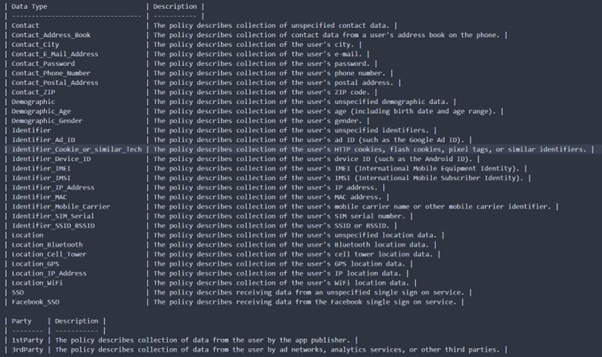
\includegraphics[width=\textwidth]{policy_classifications}

\bigskip

The APP-350 Corpus was used in a broader project to train machine learning models to conduct a privacy census of 1,035,853 Android apps. For more information about how the Corpus was annotated, see the paper “MAPS: Scaling Privacy Compliance Analysis to a Million Apps” (as attached), Section 3, Pg 69 to 70. 

\section{Rationale for utilising the APP-350 corpus} \label{sec:rationale-app350}

Since the focus of this capstone is to assess the manner in which legal analytics can transform legal practice and its corresponding limitations, this dataset was chosen for the following reasons:

\begin{enumerate}
	\item APP-350 is a labelled dataset, allowing easy validation of results. If an unlabelled dataset was used, unsupervised training would have to be conducted. The performance of the models would likely be much lower because NLP models for specific vocabulary like law are still not as sophisticated as models trained on general vocabulary. Further, there are few law specific labelled datasets.
	\item APP-350 is labelled on both the sentence and segment (i.e. paragraph) level. This provides more granular data for training the AI models. 
	\item APP-350 contains real-world data privacy practices. Thus training XAI models on such a dataset would provide a realistic insight into the extent of which AI models are explainable in the legal context.
	\item Legal tech companies are also using classification models to assist in contract / document review products. To do so, these companies train their AI models in a similar manner on similarly structured datasets. By using APP-350 to train XAI models, the results can be used as a proxy for the explainability of models that are currently used in the industry.
\end{enumerate}

\section{How Interpret Text explains predictions} \label{sec: interpret_text_exp_pred}

Interpret Text allows visualisation of the predictions of NLP models across a range of complexities. The two broad types of models that it covers are linear and tree-based models  and neural networks. For the purposes of this capstone, I will mainly be focusing on the first type of model as these models are considered “glass-box” models: A glass-box explainer implies a model that is innately explainable, where the user can fully observe and dissect the process adopted by the model in making a prediction. The hyperparameters of neural networks are much more complicated which may be too technically complicated for this capstone.

\bigskip

For linear and tree-based models, Interpret Text uses a Classical Text Explainer. The Explainer leverages this inherent explainability by exposing weights and importances over encoded tokens as explanations over each word in a document. In practice, these can be accessed through the visualization dashboard or the explanation object.

\bigskip

The explanations provided by the aforementioned glass-box methods serve as direct proxies for weights and parameters in the model, which make the final prediction.

\bigskip

This is how the visualisation dashboard looks like:

\bigskip

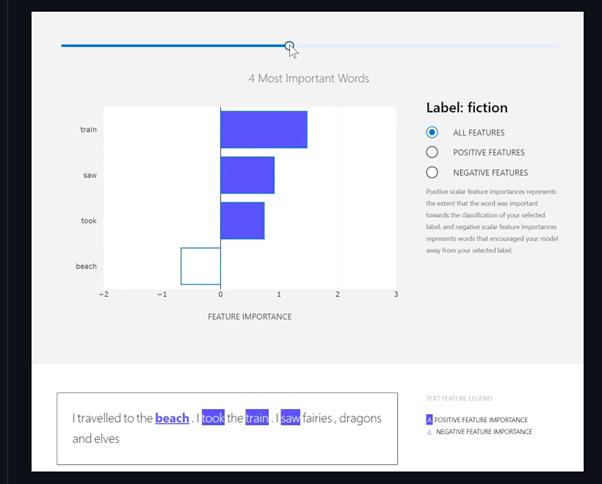
\includegraphics[width=\textwidth]{interpret_text_dashboard.png}

\bigskip

The user can visualise the top 10 important words (both positive and negative) for each label, and the dashboard provides a “weight” score for each word. The user can interact with the highlighted words to see the individual score.

\section{Model training methodology by researchers} \label{sec:model_training_method}

According to the paper “MAPS: Scaling Privacy Compliance Analysis to a Million Apps”, the researchers feature engineered the policy text as follows (Page 71 to 72): 

\begin{enumerate}
	\item Tokenisation: Lowercase all characters, remove non-ASCII characters, no stemming, normalisation of whitespace and punctuation, unigrams and bigrams.
	\item Word representation: Union of TF-IDF and manually crafted features.
	\begin{enumerate}
		\item The manually crafted features consist of Boolean values indicating the presence or absence of indicative strings the researchers observed in the data.
	\end{enumerate}
\end{enumerate}

Individual classifiers were then trained for every policy classification. For all the classifications (except for four policy classifications), they trained a model using scikitlearn SVC implementation with a linear kernel, with five-fold cross validation. For the four policy classifications, word-based rule classifiers were used instead because of the limited number of training data.

\section{Proposed model training methodology} \label{sec:proposed_training_method}

As the methodology used by the researchers seem to produce the highest performing models, I aim to replicate it. However, since Interpret Text only supports linear and tree-based classifiers, I will use the SGDClassifier instead to fit a linear SVM. I then will use Interpret Text to visualise the predictions.

\bigskip

Apart from replicating the researchers’ methodology, I will also experiment with different feature engineering approaches to compare their impact on model performance and explainability (further details to be added):

\begin{enumerate}
	\item Word representations: Bag of words and word embeddings.
	\item Different combinations of n-grams.
\end{enumerate}

I will also assess the performance and explainability of different scikitlearn linear and tree-based models (further details to be added):

\begin{enumerate}
	\item Logistic regression
	\item Ridge classifier
	\item Ada Boost
	\item Gradient Boost
	\item Random forest
\end{enumerate}

\end{document}
